% !TeX program = xelatex
\ifdefined\BookMaster\else
\documentclass[11pt,oneside]{article}
% !TeX program = xelatex
\usepackage[b5paper,left=22mm,right=22mm,top=20mm,bottom=22mm,footskip=11mm]{geometry}
\usepackage{fontspec}
\setmainfont{TeX Gyre Termes}
\setsansfont{TeX Gyre Heros}
\usepackage{amsmath,amssymb,mathtools,amsthm}
\renewcommand{\cdots}{\mathinner{\cdotp\cdotp\cdotp}}
\usepackage{graphicx,adjustbox,array,booktabs,longtable,multirow,enumitem,changepage,needspace}
\usepackage[table]{xcolor}
\usepackage{fancyhdr}
\raggedbottom
\interfootnotelinepenalty=10000
\newcommand{\BookFootnote}[2]{\begingroup\renewcommand{\thefootnote}{\fnsymbol{footnote}}\footnote[#1]{#2}\endgroup}
\newcommand{\BookFootnoteMark}[1]{\begingroup\renewcommand{\thefootnote}{\fnsymbol{footnote}}\footnotemark[#1]\endgroup}
\newcommand{\BookFootnoteText}[2]{\begingroup\renewcommand{\thefootnote}{\fnsymbol{footnote}}\footnotetext[#1]{#2}\endgroup}
\newenvironment{BookFloat}[1]{\par\addvspace{.6\baselineskip}\noindent\def\BookFloatID{#1}\begin{minipage}{\linewidth}\phantomsection\label{bookfloat:#1:start}}{\phantomsection\label{bookfloat:\BookFloatID:end}\end{minipage}\par\addvspace{.6\baselineskip}}

\usepackage[unicode,hidelinks]{hyperref}
\pagestyle{fancy}
\fancyhf{}
\newcommand{\BookFooter}{}
\fancyfoot[L]{\parbox[b]{\dimexpr\textwidth-15mm}{\footnotesize\BookFooter}}
\fancyfoot[R]{\footnotesize\thepage}
\renewcommand{\headrulewidth}{0pt}
\renewcommand{\footrulewidth}{0pt}
\setlength{\parindent}{0pt}
\setlength{\parskip}{0.2em}
\setlength{\emergencystretch}{3em}
\setlist{nosep,leftmargin=1.7em,labelsep=.65em}
\newif\ifBookNarrative
\BookNarrativetrue
\newenvironment{BookBody}{\setlength{\parindent}{0pt}}{}
\newcommand{\BookStatement}[1]{\par\addvspace{.6\baselineskip}\noindent #1\enspace\ignorespaces}
\newcommand{\BookLabel}[1]{\par\addvspace{.6\baselineskip}\needspace{3\baselineskip}\noindent\textbf{#1}\quad\ignorespaces}
\newcommand{\BookHeading}[1]{\par\addvspace{\baselineskip}\needspace{4\baselineskip}\noindent{\large\bfseries #1}\par\medskip}
\newcommand{\BookSubheading}[1]{\par\addvspace{.7\baselineskip}\needspace{3\baselineskip}\noindent{\bfseries #1}\par\smallskip}
\newcommand{\BookTextHeading}[1]{\par\addvspace{.7\baselineskip}\needspace{3\baselineskip}\noindent #1\par\smallskip}
\newcommand{\BookSectionTitle}[2]{\par\addvspace{1.2\baselineskip}\needspace{5\baselineskip}\noindent\colorbox{gray!25}{\sffamily\bfseries\small SECTION #1}\quad{\large\bfseries #2}\par\medskip}
\newcommand{\BookExerciseTitle}[1]{\par\addvspace{\baselineskip}\needspace{4\baselineskip}\noindent{\color{gray}\rule{1.5mm}{1.5mm}}\enspace{\large\bfseries Exercises #1}\par\medskip}
\newcommand{\BookBullet}[1]{\begin{list}{\textbullet}{\setlength{\leftmargin}{1.7em}\setlength{\labelwidth}{1em}\setlength{\labelsep}{.7em}\setlength{\topsep}{0pt}\setlength{\parsep}{0pt}\setlength{\itemsep}{0pt}}\item #1\end{list}}
\newcommand{\BookExercise}[2]{\begin{list}{\textbf{#1}}{\setlength{\leftmargin}{2.2em}\setlength{\labelwidth}{1.5em}\setlength{\labelsep}{.7em}\setlength{\topsep}{.15em}\setlength{\parsep}{0pt}\setlength{\itemsep}{0pt}}\item #2\end{list}}
\newcommand{\BookEnd}[1]{\unskip\nobreak\hfill\ensuremath{#1}}
\newcommand{\BookSource}[2]{\phantomsection\label{sourcepage:#1}} % Source-page anchors, retained through reflow.
\usepackage{multicol}
\usepackage{tikz}
\newcommand{\BookPartEntry}[2]{\par\noindent\makebox[17mm][l]{\bfseries Section #1}#2\par}
\newcommand{\BookPartTitle}[3]{\par\bigskip\noindent\begin{tikzpicture}\node[anchor=north west,inner sep=0pt,outer sep=0pt] (bookpart) at (0,0) {\begin{minipage}{\dimexpr\linewidth-.5pt}\hspace*{26mm}\begin{minipage}[t]{\dimexpr\linewidth-26mm}\begin{adjustbox}{max width=\linewidth}{\fontsize{20}{24}\selectfont\bfseries #2}\end{adjustbox}\par\vspace{6mm}\hrule\vspace{6mm}{\sffamily\footnotesize\setlength{\parskip}{.3em}#3}\vspace{3mm}\end{minipage}\end{minipage}};\path[shade,top color=gray!60,bottom color=white] (0,0) rectangle ([xshift=24mm]bookpart.south west);\node[anchor=north,font=\sffamily\bfseries\small] at (12mm,-2mm) {PART};\node[anchor=north,font=\sffamily\bfseries\Huge] at (12mm,-7mm) {#1};\end{tikzpicture}\par\bigskip}
\newsavebox{\BookMathBox}
\makeatletter
\newcommand{\BookInline}[1]{\leavevmode\hskip0pt\relax\begingroup\in@{\begin}{#1}\ifin@\sbox{\BookMathBox}{\(#1\)}\ifdim\wd\BookMathBox>\dimexpr\linewidth-1em\relax\resizebox{\dimexpr\linewidth-1em\relax}{!}{\usebox{\BookMathBox}}\else\(#1\)\fi\else\in@{\left}{#1}\ifin@\sbox{\BookMathBox}{\(#1\)}\ifdim\wd\BookMathBox>\dimexpr\linewidth-1em\relax\resizebox{\dimexpr\linewidth-1em\relax}{!}{\usebox{\BookMathBox}}\else\(#1\)\fi\else\(#1\)\fi\fi\endgroup\hskip0pt\relax}
\makeatother
\DeclareMathOperator{\Aut}{Aut}
\DeclareMathOperator{\End}{End}
\DeclareMathOperator{\Hom}{Hom}
\DeclareMathOperator{\GF}{GF}
\DeclareMathOperator{\irr}{irr}
\DeclareMathOperator{\lt}{lt}
\DeclareMathOperator{\lp}{lp}
\providecommand{\textcircled}[1]{\textnormal{(#1)}}

\begin{document}
\fi
\renewcommand{\BookFooter}{Section 11 Plane Isometries}
\pdfbookmark[0]{Section 11 Plane Isometries}{11_plane_isometries}
\ifdefined\BookMaster\else\setcounter{page}{105}\fi
% Source PDF page 122; original printed page 105
\BookSource{122}{105}
\BookNarrativetrue

\begin{BookBody}

\BookSectionTitle{11}{Plane Isometries\label{bookfootnote:122:2:ref}\BookFootnote{2}{\label{bookfootnote:122:2:text}This section is not used in the remainder of the text.}}

\noindent Consider the Euclidean plane \BookInline{\mathbb{R}^{2}.} An\textbf{ isometry of} \BookInline{\mathbb{R}^{2}} is a permutation \BookInline{\phi:\mathbb{R}^{2}\to \mathbb{R}^{2}} that preserves distance, so that the distance between points \BookInline{P} and \BookInline{Q} is the same as the distance between the points \BookInline{\phi (P)} and \BookInline{\phi (Q)} for all points \BookInline{P} and \BookInline{Q} in \BookInline{\mathbb{R}^{2}.} If \BookInline{\psi } is also an isometry of \BookInline{\mathbb{R}^{2},\allowbreak } then the distance between \BookInline{\psi (\phi (P))} and \BookInline{\psi (\phi (Q))} must be the same as the distance between \BookInline{\phi (P)} and \BookInline{\phi (Q),\allowbreak } which in turn is the distance between \BookInline{P} and \BookInline{Q,\allowbreak } showing that the composition of two isometries is again an isometry. Since the identity map is an isometry and the inverse of an isometry is an isometry, we see that the isometries of \BookInline{\mathbb{R}^{2}} form a subgroup of the group of all permutations of \BookInline{\mathbb{R}^{2}.}

Given any subset \BookInline{S} of \BookInline{\mathbb{R}^{2},\allowbreak } the isometries of \BookInline{\mathbb{R}^{2}} that carry \BookInline{S} onto itself form a subgroup of the group of isometries. This subgroup is the\textbf{ group of symmetries of} \BookInline{S} \textbf{in} \BookInline{\mathbb{R}^{2}.} Although we defined the dihedral group \BookInline{D_{n}} as one-to-one maps from the vertices of a regular \BookInline{n-}gon onto itself that preserves edges, we can extend each map in \BookInline{D_{n}} to an isometry of the whole plane\BookInline{;\mu } is reflection across the \BookInline{x-}axis and \BookInline{\rho } is rotation about the origin by \BookInline{\frac{2\pi }{n}}. So we can think of \BookInline{D_{n}} as the group of isometries of a regular \BookInline{n-}gon in \BookInline{\mathbb{R}^{2}.}

Everything we have defined in the two preceding paragraphs could equally well have been done for \BookInline{n-}dimensional Euclidean space \BookInline{\mathbb{R}^{n},\allowbreak } but we will concern ourselves chiefly with plane isometries here.

It can be proved that every isometry of the plane is one of just four types (see Artin [5]). We will list the types and show, for each type, a labeled figure that can be carried into itself by an isometry of that type. In each of Figs. 11.1, 11.3, and 11.4, consider the line with spikes shown to be extended infinitely to the left and to the right. We also give an example of each type in terms of coordinates.

\textit{translation} \BookInline{\tau:} Slide every point the same distance in the same direction. See Fig. 11.1. (\textit{Example}\BookInline{:\tau (x,\allowbreak y)= (x,\allowbreak y)+ (2,\allowbreak - 3)= (x+ 2,\allowbreak y- 3).)}

\textit{rotation} \BookInline{\rho:} Rotate the plane about a point \BookInline{P} through an angle \BookInline{\theta.} See Fig. 11.2. (\textit{Example}\BookInline{:\rho (x,\allowbreak y)= (- y,\allowbreak x)} is a rotation through \BookInline{90^{\circ }} counterclockwise about the origin (0, 0).)

\textit{reflection} \BookInline{\mu:} Map each point into its mirror image \BookInline{(\mu } for mirror) across a line \BookInline{L,\allowbreak } each point of which is left fixed by \BookInline{\mu.} See Fig. 11.3. The line \BookInline{L} is the\textit{ axis of} \textit{reflection}. (\textit{Example}\BookInline{:\mu (x,\allowbreak y)= (y,\allowbreak x)} is a reflection across the line \BookInline{y= x.)}

\end{BookBody}

% Source PDF page 123; original printed page 106
\BookSource{123}{106}
\BookNarrativetrue

\begin{BookBody}

\textit{glide reflection} \BookInline{\gamma:} The product of a translation and a reflection across a line mapped into itself by the translation. See Fig. 11.4. (\textit{Example}\BookInline{:\gamma (x,\allowbreak y)= (x+ 4,\allowbreak - y)} is a glide reflection along the \BookInline{x-}axis.)

Notice the little curved arrow that is carried into another curved arrow in each of Figs. 11.1 through 11.4. For the translation and rotation, the counterclockwise directions of the curved arrows remain the same, but for the reflection and glide reflection, the counterclockwise arrow is mapped into a clockwise arrow. We say that translations and rotations\textit{ preserve orientation,} while the reflection and glide reflection\textit{ reverse orien}\textit{tation}. We do not classify the identity isometry as any definite one of the four types listed; it could equally well be considered to be a translation by the zero vector or a rotation about any point through an angle of \BookInline{0^{\circ }.} We always consider a glide reflection to be the product of a reflection and a translation that is different from the identity isometry.

\begin{BookFloat}{11_plane_isometries-p123-2}
\begin{center}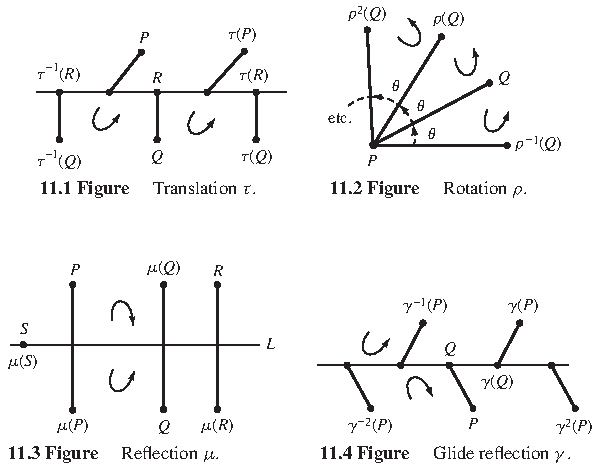
\includegraphics[width=0.819\linewidth,height=.8\textheight,keepaspectratio]{assets/p123_02.pdf}\end{center}
\end{BookFloat}

The theorem that follows describes the possible structures of finite subgroups of the full isometry group.

\BookLabel{11.5 Theorem} Every finite group \BookInline{G} of isometries of the plane is isomorphic to either the Klein 4-group, \BookInline{\mathbb{Z}_{n}} for \BookInline{n\geq 1,\allowbreak } or \BookInline{D_{n}} for some \BookInline{n\geq 3.}

\BookLabel{\textit{Proof}} \textbf{(Outline)} First we show that there is a point in the plane that is fixed by every element of \BookInline{G.} We let \BookInline{G= \{\phi _{1},\allowbreak \phi _{2},\allowbreak \phi _{3},\allowbreak...,\allowbreak \phi _{m}\}} and \BookInline{(x_{i},\allowbreak y_{i})= \phi _{i}(0,\allowbreak 0).} Then the point

\begin{center}\begin{adjustbox}{max width=\linewidth}\BookInline{\displaystyle P = (\overline{x},\allowbreak  \overline{y}) = \left( \frac{x_1 + x_2 + x_3 + \cdots + x_m}{m},\allowbreak  \frac{y_1 + y_1 + y_3 + \cdots + y_m}{m} \right)}\end{adjustbox}\end{center}

\noindent is the center of mass of the set \BookInline{S= \{(x_{i},\allowbreak y_{i})\mid 1\leq i\leq m\}} where each point is weighted by the number of \BookInline{\phi _{i}} that map (0, 0) to that point. It is easy to see that the isometries in \BookInline{G} permute the points in \BookInline{S} since for each \BookInline{i} and \BookInline{j,\allowbreak \phi _{i}\circ \phi _{j}= \phi _{k}} for some \BookInline{k.} Thus \BookInline{\phi _{i}(x_{j},\allowbreak y_{j})= } \BookInline{(x_{k},\allowbreak y_{k}).} This implies the center of mass of \BookInline{\phi (S)} is the same as the center of mass of \BookInline{S.} It can be shown that given the distances from the center of mass to the points of the set \BookInline{S,\allowbreak } the center of mass is the only point having these distances from the points of \BookInline{S.} This says that \BookInline{(x,\allowbreak y)} is fixed by every isometry in \BookInline{G.}

\end{BookBody}

% Source PDF page 124; original printed page 107
\BookSource{124}{107}
\BookNarrativetrue

\begin{BookBody}

The orientation preserving isometries of \BookInline{G} form a subgroup \BookInline{H} of \BookInline{G} which is either all of \BookInline{G} or else of order \BookInline{m/2.} You are asked to prove this in Exercise 22. Of course \BookInline{H} consists of the identity and possibly rotations about the point \BookInline{(x,\allowbreak y).} If \BookInline{H} has only one element, then \BookInline{G} has one or two elements and is therefore isomorphic with \BookInline{\mathbb{Z}_{1}} or \BookInline{\mathbb{Z}_{2}.} If \BookInline{H} has two elements, then \BookInline{G} has two or four elements and is therefore isomorphic with either the Klein 4-group\BookInline{,\allowbreak \mathbb{Z}_{4},\allowbreak } or \BookInline{\mathbb{Z}_{2}.} So we can assume that \BookInline{H} has at least three elements.

If we choose a rotation \BookInline{\rho } in \BookInline{H} that rotates through the smallest positive angle \BookInline{\theta } among all the elements of \BookInline{H,\allowbreak \rho } generates \BookInline{H.} The proof of this fact is similar to the proof that a subgroup of a cyclic group is cyclic and you are asked to provide the details of the proof in Exercise 23. If \BookInline{G= H,\allowbreak } then \BookInline{G} is isomorphic with \BookInline{\mathbb{Z}_{m}.} So we now assume that \BookInline{G} contains a reflection, say \BookInline{\mu.} Then the coset \BookInline{\mu H} contains only isometries of \BookInline{G} that reverse orientation. Each coset \BookInline{H} and \BookInline{\mu H} contains half the elements of \BookInline{G,\allowbreak } so \BookInline{G= H\cup \mu H.}

Consider now a regular \BookInline{n-}gon (recall that we are assuming that \BookInline{n\geq 3)} with center the point \BookInline{(x,\allowbreak y)} and having a vertex \BookInline{v_{0}} on the line fixed by \BookInline{\mu.} Each element of \BookInline{G} permutes the vertices of the \BookInline{n-}gon and preserves edges. Furthermore, no two elements of \BookInline{G} permute the vertices in the same way. Thus \BookInline{G} is isomorphic with a subgroup of the dihedral group \BookInline{D_{n}.} Since \BookInline{|G|= |D_{n}|,\allowbreak G} is isomorphic with \BookInline{D_{n}.}\BookEnd{\blacklozenge}

In Theorem 11.5 the Klein 4-group\BookInline{,\allowbreak V,\allowbreak } seems like an exception. However\BookInline{,\allowbreak V} fits into the family of dihedral groups since \BookInline{V} has two elements of order \BookInline{2,\allowbreak a} and \BookInline{b,\allowbreak } with the property that \BookInline{ab= ba^{- 1}.} Sometimes \BookInline{V} is denoted \BookInline{D_{2}} and considered a dihedral group. The isometries of the plane that map a line segment to itself are isomorphic with \BookInline{V.}

The preceding theorem gives the complete story about finite plane isometry groups. We turn now to some infinite groups of plane isometries that arise naturally in decorating and art. Among these are the\textit{ discrete frieze groups}. A discrete frieze consists of a pattern of finite width and height that is repeated endlessly in both directions along its baseline to form a strip of infinite length but finite height; think of it as a decorative border strip that goes around a room next to the ceiling on wallpaper. We consider those isometries that carry each basic pattern onto itself or onto another instance of the pattern in the frieze. The set of all such isometries is called the\textbf{ “frieze group.”} All discrete frieze groups are infinite and have a subgroup isomorphic to \BookInline{\mathbb{Z}} generated by the translation that slides the frieze lengthwise until the basic pattern is superimposed on the position of its next neighbor pattern in that direction. As a simple example of a discrete frieze, consider integral signs spaced equal distances apart and continuing infinitely to the left and right, indicated schematically like this.

\begin{BookFloat}{11_plane_isometries-p124-5}
\begin{center}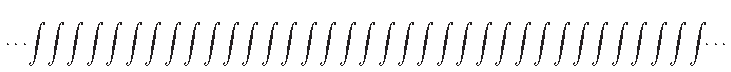
\includegraphics[width=1.000\linewidth,height=.8\textheight,keepaspectratio]{assets/p124_05.pdf}\end{center}
\end{BookFloat}

\noindent Let us consider the integral signs to be one unit apart. The symmetry group of this frieze is generated by a translation \BookInline{\tau } sliding the plane one unit to the right, and by a rotation \BookInline{\rho } of \BookInline{180^{\circ }} about a point in the center of some integral sign. There are no horizontal or vertical reflections, and no glide reflections. This frieze group is nonabelian; we can check that \BookInline{\tau \rho = \rho \tau ^{- 1}.} This relation between \BookInline{\tau } and \BookInline{\rho } looks very familiar. The dihedral group \BookInline{D_{n}} is also generated by two elements \BookInline{\rho } and \BookInline{\mu } that satisfy the relation \BookInline{\rho \mu = \mu \rho ^{- 1}.} If \BookInline{\tau } and \BookInline{\rho } in the frieze group are replaced by \BookInline{\rho } and \BookInline{\mu,\allowbreak } respectively, we have the same relation. In \BookInline{D_{n},\allowbreak \mu } has order 2, as does \BookInline{\rho } in the frieze group, but the element \BookInline{\rho } in \BookInline{D_{n}} has order \BookInline{n} while \BookInline{\tau } has infinite order. Thus it is natural to use the notation \BookInline{D_{\infty }} for this nonabelian frieze group.

As another example, consider the frieze given by an infinite string of D’s.

\BookTextHeading{\ensuremath{\cdot} \ensuremath{\cdot} \ensuremath{\cdot} \textbf{D D D D D D D D D D D}\ensuremath{\cdot} \ensuremath{\cdot} \ensuremath{\cdot}    }

\end{BookBody}

% Source PDF page 125; original printed page 108
\BookSource{125}{108}
\BookNarrativetrue

\begin{BookBody}

\noindent Its group is generated by a translation \BookInline{\tau } one step to the right and by a vertical reflection \BookInline{\mu } across a horizontal line cutting through the middle of all the D’s. We can check that these group generators commute this time, that is\BookInline{,\allowbreak \tau \mu = \mu \tau,\allowbreak } so this frieze group is abelian and is isomorphic to \BookInline{\mathbb{Z}\times \mathbb{Z}_{2}.}

It can be shown that if we classify such discrete friezes only by whether or not their groups contain a

\begin{center}\begin{adjustbox}{max width=\linewidth}\BookInline{\displaystyle \begin{aligned}&\;\text{rotation horizontal axis re}\;\text{fl}\;\text{ection}\; \\ &\;\text{vertical axis re}\;\text{fl}\;\text{ection nontrivial glide re}\;\text{fl}\;\text{ection}\;\end{aligned}}\end{adjustbox}\end{center}

\noindent then there are a total of seven possibilities. A\textit{ nontrivial glide reflection} in a symmetry group is one that is not equal to a product of a translation in that group and a reflection in that group. The group for the string of D’s above contains glide reflections across the horizontal line through the centers of the D’s, but the translation component of each glide reflection is also in the group so they are all considered trivial glide reflections in that group. The frieze group for

\begin{BookFloat}{11_plane_isometries-p125-4}
\begin{center}
\includegraphics[width=1.000\linewidth,height=.8\textheight,keepaspectratio]{assets/p125_04.pdf}\end{center}
\end{BookFloat}

\noindent contains a nontrivial glide reflection whose translation component is not an element of the group. The exercises exhibit the seven possible cases, and ask you to tell, for each case, which of the four types of isometries displayed above appear in the symmetry group. We do not obtain seven different group structures. Each of the groups obtained can be shown to be isomorphic to one of

\begin{center}\begin{adjustbox}{max width=\linewidth}\BookInline{\displaystyle \mathbb{Z},\allowbreak D_{\infty },\allowbreak \mathbb{Z}\times \mathbb{Z}_{2},\allowbreak \;\text{or}\;D_{\infty }\times \mathbb{Z}_{2}.}\end{adjustbox}\end{center}

Equally interesting is the study of symmetries when a pattern in the shape of a square, parallelogram, rhombus, or hexagon is repeated by translations along\textit{ two non}\textit{parallel vector directions} to fill the entire plane, like patterns that appear on wallpaper. These groups are called the\textit{ wallpaper groups} or the\textit{ plane crystallographic groups}. While a frieze could not be carried into itself by a rotation through a positive angle less than \BookInline{180^{\circ },\allowbreak } it is possible to have rotations of \BookInline{60^{\circ },\allowbreak 90^{\circ },\allowbreak 120^{\circ },\allowbreak } and \BookInline{180^{\circ }} for some of these plane-filling patterns. Figure 11.6 provides an illustration where the pattern consists of a square. We are interested in the group of plane isometries that carry this square onto itself or onto another square. Generators for this group are given by two translations (one sliding a square to the next neighbor to the right and one to the next above), by a rotation through \BookInline{90^{\circ }} about the center of a square, and by a reflection in a vertical (or horizontal) line along the edges of the square. The one reflection is all that is needed to “turn the plane over”; a diagonal reflection can also be used. After being turned over, the translations and rotations can be used again. The isometry group for this\textit{ periodic} \textit{pattern} in the plane surely contains a subgroup isomorphic to \BookInline{\mathbb{Z}\times \mathbb{Z}} generated by the unit translations to the right and upward, and a subgroup isomorphic to \BookInline{D_{4}} generated by those isometries that carry one square (it can be any square) into itself.

If we consider the plane to be filled with parallelograms as in Fig. 11.7, we do not get all the types of isometries that we did for Fig. 11.6. The symmetry group this time is generated by the translations indicated by the arrows and a rotation through \BookInline{180^{\circ }} about any vertex of a parallelogram.

It can be shown that there are 17 different types of wallpaper patterns when they are classified according to the types of rotations, reflections, and nontrivial glide reflections that they admit. We refer you to Gallian [8] for pictures of these 17 possibilities and a chart to help you identify them. The exercises illustrate a few of them. The situation

\end{BookBody}

% Source PDF page 126; original printed page 109
\BookSource{126}{109}
\BookNarrativetrue

\begin{BookBody}

\begin{BookFloat}{11_plane_isometries-p126-0}
\begin{center}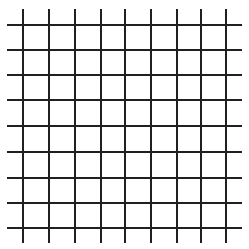
\includegraphics[width=0.341\linewidth,height=.8\textheight,keepaspectratio]{assets/p126_00.pdf}\end{center}
\begin{center}\small\textbf{11.6 Figure}\end{center}
\end{BookFloat}

\begin{BookFloat}{11_plane_isometries-p126-1}
\begin{center}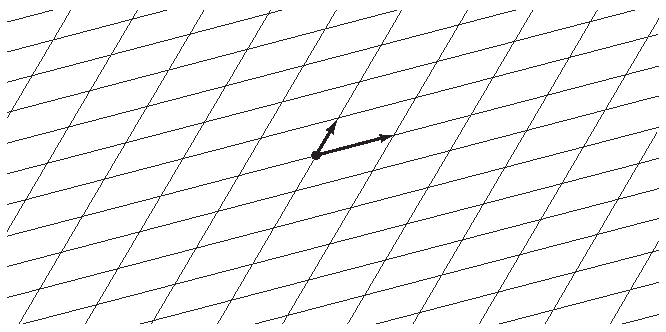
\includegraphics[width=0.913\linewidth,height=.8\textheight,keepaspectratio]{assets/p126_02.pdf}\end{center}
\begin{center}\small\textbf{11.7 Figure}\end{center}
\end{BookFloat}

\noindent in space is more complicated; it can be shown that there are 230 three-dimensional crystallographic groups. The final exercise we give involves rotations in space.

M. C. Escher (1898–1973) was an artist whose work included plane-filling patterns. In the exercises you are asked to analyze two of his works of this type.

\end{BookBody}

\BookNarrativefalse

\begin{BookBody}

\BookExerciseTitle{11}

\BookExercise{1.}{This exercise shows that the group of symmetries of a certain type of geometric figure may depend on the dimension of the space in which we consider the figure to lie.}

\BookExercise{a.}{Describe all symmetries of a point in the real line \BookInline{\mathbb{R};} that is, describe all isometries of \BookInline{\mathbb{R}} that leave one point fixed.}

\BookExercise{b.}{Describe all symmetries (translations, reflections, etc.) of a point in the plane \BookInline{\mathbb{R}^{2}.}}

\BookExercise{c.}{Describe all symmetries of a line segment in \BookInline{\mathbb{R}.}}

\BookExercise{d.}{Describe all symmetries of a line segment in \BookInline{\mathbb{R}^{2}.}}

\BookExercise{e.}{Describe some symmetries of a line segment in \BookInline{\mathbb{R}^{3}.}}

\BookExercise{2.}{Let \BookInline{P} stand for an orientation preserving plane isometry and \BookInline{R} for an orientation reversing one. Fill in the table with \BookInline{P} or \BookInline{R} to denote the orientation preserving or reversing property of a product.}

\end{BookBody}

% Source PDF page 127; original printed page 110
\BookSource{127}{110}
\BookNarrativefalse

\begin{BookBody}

\begin{BookFloat}{11_plane_isometries-p127-0}
\begin{center}\begin{adjustbox}{max width=\linewidth}
\renewcommand{\arraystretch}{1.2}\setlength{\tabcolsep}{5pt}
\begin{tabular}{c|c|c}
 & \BookInline{P} & \BookInline{R}\\\hline
\BookInline{P} &  & \\\hline
\BookInline{R} &  & \\
\end{tabular}
\end{adjustbox}\end{center}
\end{BookFloat}

\BookExercise{3.}{Fill in the table to give\textit{ all} possible types of plane isometries given by a product of two types as indicated in Tables 11.1 through 11.4. For example, a product of two rotations may be a rotation, or it may be another type. Fill in the box corresponding to \BookInline{\rho \rho } with both letters. Use your answer to Exercise 2 to eliminate some types. Eliminate the identity from consideration.}

\begin{BookFloat}{11_plane_isometries-p127-2}
\begin{center}\begin{adjustbox}{max width=\linewidth}
\renewcommand{\arraystretch}{1.2}\setlength{\tabcolsep}{5pt}
\begin{tabular}{c|c|c|c|c}
 & \BookInline{\tau } & \BookInline{\rho } & \BookInline{\mu } & \BookInline{\gamma }\\\hline
\BookInline{\tau } &  &  &  & \\\hline
\BookInline{\rho } &  &  &  & \\\hline
\BookInline{\mu } &  &  &  & \\\hline
\BookInline{\gamma } &  &  &  & \\
\end{tabular}
\end{adjustbox}\end{center}
\end{BookFloat}

\BookExercise{4.}{Draw a plane figure that has a one-element group as its group of symmetries in \BookInline{\mathbb{R}^{2}.}}

\BookExercise{5.}{Draw a plane figure that has a two-element group as its group of symmetries in \BookInline{\mathbb{R}^{2}.}}

\BookExercise{6.}{Draw a plane figure that has a three-element group as its group of symmetries in \BookInline{\mathbb{R}^{2}.}}

\BookExercise{7.}{Draw a plane figure that has a four-element group isomorphic to \BookInline{\mathbb{Z}_{4}} as its group of symmetries in \BookInline{\mathbb{R}^{2}.}}

\BookExercise{8.}{Draw a plane figure that has a four-element group isomorphic to the Klein 4-group \BookInline{V} as its group of symmetries in \BookInline{\mathbb{R}^{2}.}}

\BookExercise{9.}{For each of the four types of plane isometries (other than the identity), give the possibilities for the order of an isometry of that type in the group of plane isometries.}

\BookExercise{10.}{A plane isometry \BookInline{\phi } has a \BookInline{\text{fi}xed} \textit{point} if there exists a point \BookInline{P} in the plane such that \BookInline{\phi (P)= P.} Which of the four types of plane isometries (other than the identity) can have a fixed point?}

\BookExercise{11.}{Referring to Exercise 10, which types of plane isometries, if any, have exactly one fixed point?}

\BookExercise{12.}{Referring to Exercise 10, which types of plane isometries, if any, have exactly two fixed points?}

\BookExercise{13.}{Referring to Exercise 10, which types of plane isometries, if any, have an infinite number of fixed points?}

\BookExercise{14.}{Argue geometrically that a plane isometry that leaves three noncolinear points fixed must be the identity map.}

\BookExercise{15.}{Using Exercise 14, show algebraically that if two plane isometries \BookInline{\phi } and \BookInline{\psi } agree on three noncolinear points, that is, if \BookInline{\phi (P_{i})= \psi (P_{i})} for noncolinear points \BookInline{P_{1},\allowbreak P_{2},\allowbreak } and \BookInline{P_{3},\allowbreak } then \BookInline{\phi } and \BookInline{\psi } are the same map.}

\BookExercise{16.}{Do the rotations, together with the identity map, form a subgroup of the group of plane isometries? Why or why not?}

\BookExercise{17.}{Do the translations, together with the identity map, form a subgroup of the group of plane isometries? Why or why not?}

\BookExercise{18.}{Do the rotations about one particular point \BookInline{P,\allowbreak } together with the identity map, form a subgroup of the group of plane isometries? Why or why not?}

\BookExercise{19.}{Does the reflection across one particular line \BookInline{L,\allowbreak } together with the identity map, form a subgroup of the group of plane isometries? Why or why not?}

\BookExercise{20.}{Do the glide reflections, together with the identity map, form a subgroup of the group of plane isometries? Why or why not?}

\BookExercise{21.}{Which of the four types of plane isometries can be elements of a\textit{ finite} subgroup of the group of plane isometries?}

\BookExercise{22.}{Completing a detail of the proof of Theorem 11.5, let \BookInline{G} be a finite group of plane isometries. Show that the rotations in \BookInline{G,\allowbreak } together with the identity isometry, form a subgroup \BookInline{H} of \BookInline{G,\allowbreak } and that either \BookInline{H= G} or \BookInline{|G|= 2|H|.[}\textit{Hint:} Use the same method that we used to show that \BookInline{|S|= 2|A|.]}}

\end{BookBody}

% Source PDF page 128; original printed page 111
\BookSource{128}{111}
\BookNarrativefalse

\begin{BookBody}

\BookExercise{23.}{Completing a detail in the proof of Theorem 11.5, let \BookInline{G} be a finite group consisting of the identity isometry and rotations about one point \BookInline{P} in the plane. Show that \BookInline{G} is cyclic, generated by the rotation in \BookInline{G} that turns the plane counterclockwise about \BookInline{P} through the smallest angle \BookInline{\theta >0.[}\textit{Hint:} Follow the idea of the proof that a subgroup of a cyclic group is cyclic.]}

\noindent Exercises 24 through 30 illustrate the seven different types of friezes when they are classified according to their symmetries. Imagine the figure shown to be continued infinitely to the right and left. The symmetry group of a frieze always contains translations. For each of these exercises answer these questions about the symmetry group of the frieze.

\BookExercise{a.}{Does the group contain a rotation?}

\BookExercise{b.}{Does the group contain a reflection across a horizontal line?}

\BookExercise{c.}{Does the group contain a reflection across a vertical line?}

\BookExercise{d.}{Does the group contain a nontrivial glide reflection?}

\BookExercise{e.}{To which of the possible groups \BookInline{\mathbb{Z},\allowbreak D_{\infty },\allowbreak \mathbb{Z}\times \mathbb{Z}_{2},\allowbreak } or \BookInline{D_{\infty }\times \mathbb{Z}_{2}} do you think the symmetry group of the frieze is isomorphic?}

\BookExercise{24.}{\textbf{ F F F F F F F F F F F F F F F}}

\BookExercise{25.}{\textbf{ T T T T T T T T T T}}

\BookExercise{26.}{\textbf{ E E E E E E E E E E E E}}

\BookExercise{27.}{\textbf{ Z Z Z Z Z Z Z Z Z Z Z Z}}

\BookExercise{28.}{\textbf{ H H H H H H H H H H}}

\begin{BookFloat}{11_plane_isometries-p128-12}
\begin{center}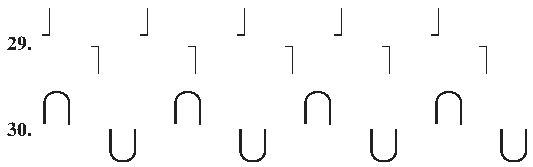
\includegraphics[width=0.731\linewidth,height=.8\textheight,keepaspectratio]{assets/p128_08.pdf}\end{center}
\end{BookFloat}

\noindent Exercises 31 through 37 describe a pattern to be used to fill the plane by translation in the two directions given by the specified vectors. Answer these questions in each case.

\BookExercise{a.}{Does the symmetry group contain any rotations? If so, through what possible angles \BookInline{\theta } where \BookInline{0<\theta \leq } \BookInline{180^{\circ }}?}

\BookExercise{b.}{Does the symmetry group contain any reflections?}

\BookExercise{c.}{Does the symmetry group contain any nontrivial glide reflections?}

\BookExercise{31.}{A square with horizontal and vertical edges using translation directions given by vectors (1, 0) and (0, 1).}

\BookExercise{32.}{A square as in Exercise 31 using translation directions given by vectors \BookInline{(1,\allowbreak 1/2)} and (0, 1).}

\BookExercise{33.}{A square as in Exercise 31 with the letter L at its center using translation directions given by vectors (1, 0) and (0, 1).}

\BookExercise{34.}{A square as in Exercise 31 with the letter E at its center using translation directions given by vectors (1, 0) and (0, 1).}

\BookExercise{35.}{A square as in Exercise 31 with the letter H at its center using translation directions given by vectors (1, 0) and (0, 1).}

\BookExercise{36.}{A regular hexagon with a vertex at the top using translation directions given by vectors (1, 0) and \BookInline{(1,\allowbreak \sqrt{3}).}}

\BookExercise{37.}{A regular hexagon with a vertex at the top containing an equilateral triangle with vertex at the top and centroid at the center of the hexagon, using translation directions given by vectors (1, 0) and \BookInline{(1,\allowbreak \sqrt{3}).}}

\noindent Exercises 38 and 39 are concerned with art works of M. C. Escher. Find images of the indicated art by searching on the internet. Neglect the shading and colors in the figures and assume the markings in each human figure, reptile, 
% Source PDF page 129; original printed page 112
\BookSource{129}{112}
or horseman are the same, even though they may be invisible due to shading. Answer the same questions (a), (b), and (c) that were asked for Exercises 31 through 36, and also answer this part (d).

\end{BookBody}

\BookNarrativefalse

\begin{BookBody}

\BookExercise{d.}{Assuming horizontal and vertical coordinate axes with equal scales as usual, give vectors in the two nonparallel directions of vectors that generate the translation subgroup. Do not concern yourself with the length of these vectors.}

\BookExercise{38.}{\textit{ The Study of Regular Division of the Plane with Horsemen}.}

\BookExercise{39.}{\textit{ The Study of Regular Division of the Plane with Reptiles}.}

\BookExercise{40.}{Let \BookInline{\phi:\mathbb{R}\to U} be given by \BookInline{\phi (\theta )= } cos\BookInline{(\theta )+ i} sin\BookInline{(\theta )} and \BookInline{S= \phi [\mathbb{Z}].}}

\BookExercise{a.}{Show that any rotation mapping \BookInline{S} to \BookInline{S} is a rotation by an angle \BookInline{n\in \mathbb{Z}} where angles are measured in radians. \textbf{b.} Show that reflection across the \BookInline{x-}axis maps \BookInline{S} to \BookInline{S.}}

\BookExercise{c.}{What is the group of symmetries of \BookInline{S}?}

\BookExercise{41.}{Show that the rotations of a cube in space form a group isomorphic to \BookInline{S_{4}.[}\textit{Hint:} A rotation of the cube permutes the diagonals through the center of the cube.]}

\end{BookBody}
\ifdefined\BookMaster\let\BookFinish\relax\else\def\BookFinish{\end{document}}\fi\BookFinish
